\DiaryEntry{Game Theory, I}{2023-10-10}{Game Theory}

Initially started with \cite{Maschler2013}, but then switched over to \cite{Watson2013} (better and clearer explanation, simpler notation).

Game theory uses mathematical tools to model and analyze situations of interactive decision making. The situations involve several decision makers (called players) with different goals, in which the decision of each affects the outcome for all the decision makers.

This interactivity distinguishes game theory from standard decision theory. Game theory tries to predict the behavior of the players and sometimes also provides decision makers with suggestions regarding ways in which they can achieve their goals.

\subsection{Extensive-Form Games}

We need a complete description of a game and this should contain the following elements:

\begin{itemize}
\item A set of players,
\item The possible actions available to each player,
\item Rules determining the order in which players make their moves,
\item A rule determining when the game ends,
\item A rule determining the outcome of every possible game ending.
\end{itemize}

A comprehensive description is by means of a tree where every player’s action is depicted as a transition from one vertex to another vertex.

\paragraph{Example.} As a simple example consider a game with two players, I and II, which play on a $2 \times 2$ gameboard as depicted in the following Figure.

\begin{figure}[H]
    \centering
    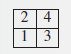
\includegraphics[scale=1.2]{images/2023-10-10-game_theory_01.png}
\end{figure}

Player I has the opening move, in which he "captures" one of the squares. By alternate turns, each player captures one of the squares, subject to the following conditions:

\begin{itemize}
	\item A square may be captured by a player only if it has not been previously captured by either player.
	\item Square 4 may not be captured if square 2 or square 3 has been previously captured.
	\item The game ends when square 1 is captured. The player who captures square 1 is the losing player.
\end{itemize}

Intuitively spoken, each player tries to froce the other to capture square 1 in order to win the game.

We can represent the game in extensive-form with the following graph. Every circled vertex represents a decision by a player, and is labeled with the number of that player. The terminal vertices of the game are indicated by dark dots. The edges of the graph depict game actions. The number that appears next to each edge corresponds to the square that is captured. Next to every terminal vertex, the corresponding game outcome is indicated. A game depicted by such a graph is called a \emph{game in extensive form}, or \emph{extensive-form game}.

\begin{figure}[H]
    \centering
    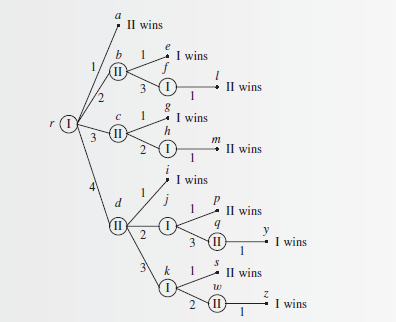
\includegraphics[scale=1.2]{images/2023-10-10-game_theory_02.png}
\end{figure}

The graph starts in vertex $r$ where player I can choose to capture any of the $4$ squares. Chosing square $1$ brings us to vertex $a$ which corresponds to a loss of player I. Chosing square $2$ brings us to vertex $b$ where player II has two options: Either capture square $1$ (vertext $e$) in which case player I wins, or capture square $3$ which brings us to vertex $f$. Here the only option for player I is to capture square $1$ which results in the victory of player II.

Based on above example, we state that various games can be represented by trees: The root of the tree corresponds to the initial position of the game, and every game position is represented by a vertex of the tree. The children of each vertex $v$ are the vertices corresponding to the game positions that can be arrived at from $v$ via one action. In other words, the number of children of a vertex is equal to the number of possible actions in the game position corresponding to that vertex. For every vertex that is not a leaf, we need to specify the player who is to take an action at that vertex. At each leaf, we need to describe the outcome of the game.

\begin{definition}
The formal definition of a game in extensive form is an ordered vector $\Gamma$,

\bee
\Gamma = (N, V, E, x^0, (V_i)_{i \in N}, O, u)
\eee

where

\begin{itemize}
	\item $N$ is finite set of players,
	\item $(V, E, x^0)$ describes the game tree (with vertex set $V$, edge set $E$, and root vertex $x^0$),
	\item $(V_i)_{i \in N}$ is a partition of the set of vertices that are not leaves,
	\item $O$ is the set of possible game outcomes.
	\item $u$ is a function associating every leaf of the tree with a game outcome in the set $O$.
\end{itemize}

\end{definition}

For each player $i \in N$, the set $V_i$ is player $i$’s set of decision vertices. For each leave $x$, the outcome at that leave is $u(x)$.

Note that the partition $V_i$ may contain empty sets. We accept the possibility of empty sets in order to be able to treat games in which a player may not be required to make any moves, but is still a game participant who is affected by the outcome of the game.

In the example game above, the various sets have the following elements

\begin{align*}
N &= \{I, II\}	\\
V &= \{r, a, b, c, d, e, f, g, h, i, j, k, l, m, p, q, s, w, y, z\}	\\
x^0 &= r \\
V_I &= \{r, f, h, j, k\} \\
V_{II} &= \{b, c, d, q, w\}
\end{align*}

The set of possible outcomes is $O = \{I \text{ wins}, II \text{ wins} \}$, and the function $u$ is given by

\begin{align*}
u(a) &= u(l) = u(m) = u(p) = u(s) = \text{ II wins} \\
u(e) &= u(g) = u(i) = u(y) = u(z) = \text{ I wins} \qed
\end{align*}

Finally, denote by $C(x)$ the set of all children of a non-leaf vertex $x$. Every edge that leads from $x$ to one of its children is called a possible action at $x$. We will associate every action with the child to which it is connected, and denote by $A(x)$ the set of all actions that are possible at the vertex $x$.

By definition, the collection of the vertices of the graph is a finite set, so that the game necessarily ends at a leaf, yielding a sequence of vertices $(x^0, x^1, \ldots , x^k)$, where $x^0$ is the root of the tree, $x^k$ is a leaf, and $x^{l+1} \in C(x^l)$ for $l = 0, 1, \ldots k-1$. This sequence is called a play. Every play ends at a particular leaf $x^k$ with outcome $u(x^k)$. Similarly, every leaf $x^k$ determines a unique play, which corresponds to the unique path connecting the root $x^0$ with $x^k$.

It follows from the above description that every player who is to take an action knows the current state of the game, meaning that he knows all the actions in the game that led to the current point in the play. This implicit assumption is called \emph{perfect information}.

Above definitions are for finite games. There are also \emph{inifinite games}, where the game tree $(V, E, x^0)$ is infinite. This can happen in two possible ways: (i) It is possible that the depth of the tree is bounded, i.e., that there exists a natural number $L$ such that the length of every path in the tree is less than or equal to $L$. This corresponds to a game that ends after at most $L$ actions have been played, and there is at least one player who has an infinite number of actions available at an information set. (ii) It is possible, that the depth of the vertices of the tree is not bounded; that is, there exists an infinite path in the game tree. This corresponds to a game that might never end.


With all these formal definition in place, we can now define one of the central concepts of game theory: the strategy.

\begin{definition}
A strategy for player $i$ is a function $s_i$ mapping each vertex $x \in V_i$ to an element in $A(x)$ (equivalently, to an element in $C(x)$).
\end{definition}

According to this definition, a strategy includes instructions on how to behave at each vertex in the game tree, including vertices that previous actions by the player preclude from being reached.

We consider the following game for two players: Player 1 decides between “out” (O) and “in” (I). If he chooses O, then the game ends with a payoff vector of $(2, 2)$. If he selects I, then player 2 is faced with the same two choices. If player 2 then chooses O, the game ends with the payoff vector $(1, 3)$. If she picks I, then player 1 has another choice to make, between A and B (ending the game with payoffs $(4, 2)$ and $(3, 4)$, respectively). 

\begin{figure}[H]
    \centering
    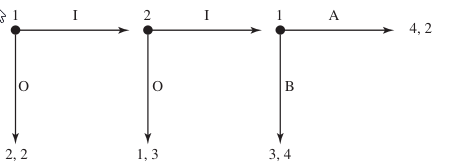
\includegraphics[scale=0.7]{images/2023-10-10-game_theory_02a.png}
\end{figure}

Player 1 has to take two decisions, whereas layer 2 has one. Note that in this game, player l’s strategy must specify what he will do at the beginning of the game (O or I) \emph{and} what action he would take at his second decision point (A or B) -- even if he may not reach this second decision point (because his first decision was O). There are four combinations of the two actions at each information set, and so there are four different strategies for player 1: OA, OB, IA, and IB.

This shows that a strategy is a  “complete contingent plan” and this means more than just a “plan” for how to play the game. If player 1 choses O at the first decision, he will not reach the second decision point. Nevertheless, the strategy (according to definition) requires a specification of player l’s choice at his second decision point even in the situation in which he plans to select O at his first decision.

We will need to keep track of behavior at all decision points -- even those that would be unreached if players follow their strategies -- to fully analyze any game. That is, stating that player l’s plan is O does not provide enough information for us to conduct a thorough analysis.



\subsection{Normal Form Representation (Strategic Form Representation)}

The extensive form is one straightforward way of representing a game. Another way of formally describing games is based on the idea of strategies. It is called the \emph{normal form} (or strategic form) representation of a game. This alternative representation is more compact than the extensive form in some settings.

For any game in extensive form, we can describe the strategy spaces of the players. Furthermore, notice that each strategy profile fully describes how the game is played. That is, a strategy profile tells us exactly what path through the tree is followed and which terminal node is reached to end the game. Associated with each terminal node (which we may call an outcome) is a payoff vector for the players. For each player $i$, we can define a \emph{payoff function} $u_i: S \rightarrow \mR$, which assigns each strategy profile $s \in S$ to player $i$'s payoff in the game. 

In the previous example, the strategy profiles $S$ are

\bee
S = \{(OA, O),  (OA, I), (OB, O), (OB, I), (IA, O), (IA, I), (IB, O), (IB, I)\}
\eee

The players’ payoff functions are defined over S. To determine $u_i(s)$ for any strategy profile $s$, start at the initial node and trace through the tree
according to the actions specified by this strategy profile. For instance, $u_1(OA, O) = 2, u_1(IA, I) = 4, u_2(IA, O) = 3$, and so forth.

For two-player games in which each player has a finite number of strategies, we can use a matrix: Each row of the matrix corresponds to a strategy of player 1, and each column corresponds to a strategy of player 2. Thus each cell of the matrix corresponds to a strategy profile. Inside a given cell, we write the payoff vector associated with the strategy profile.

In the example from above, this matrix is shown in the following Figure.


\begin{figure}[H]
    \centering
    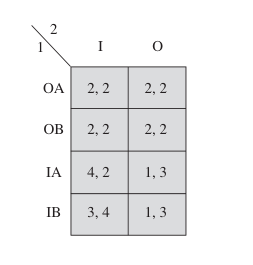
\includegraphics[scale=0.7]{images/2023-10-10-game_theory_03a.png}
\end{figure}


\subsection{Some Classical (Normal-form) Games}

\paragraph{Game of matching Pennies.} Two players simultaneously and independently select “heads” or “tails” by each uncovering a penny in his hand. If their selections match, then player 2 must give his penny to player 1; otherwise, player 1 gives his penny to player 2.

\paragraph{Coordination Game.} Both players obtain a positive payoff if they select the same strategy; otherwise they get nothing. The “Pareto coordination” game has the added feature that both players prefer to coordinate on strategy A rather than on strategy B.

\paragraph{Prisoners’ Dilemma.} The authorities have captured two criminals who they know are guilty of a certain crime. However, the authorities have only enough evidence to convict them of a minor offense. If neither crook admits to the crime, then both will be charged with the minor offense and will pay a moderate fine. The authorities have put the prisoners into separate rooms, where each prisoner is asked to squeal on the other. Squealing corresponds to strategy D (defect), and not squealing corresponds to strategy C (cooperate with the other prisoner).

Each is told that if he squeals and the other prisoner does not, then he will be granted immunity and be released; his testimony, however, will be used to convict the other prisoner of the crime. If each squeals on the other, then they both get sent to jail, but their term is reduced because of their cooperation. The best outcome for a prisoner is to defect while the other cooperates (payoff 3); the next-best outcome occurs when neither defects (payoff 2 ; then comes the outcome in which both defect (payoff 1); the worst outcome for a prisoner is when he cooperates while the other defects.

\paragraph{Battle of the Sexes.} Two friends have to decide whether to see a movie or go to the opera. Unfortunately, they work in different parts of the city and cannot communicate with each other. Therefore, they must simultaneously and independently select an event to attend. There is only one movie theater and only one opera venue, so the friends will meet each other if they manage to coordinate their decisions. Both prefer to be together, regardless of which event they attend. However, player 1 prefers the opera and player 2 prefers the movie.

\paragraph{Game of Chicken.} Two players drive automobiles toward each other at top speed. Just before they reach each other, each chooses between maintaining course (H) and swerving (D). If both swerve, they both save face and are satisfied. If only one swerves, then he is proved to be a wimp, whereas the other is lauded as a tough guy with steely nerves. If both maintain course, they crash and lose both.

\paragraph{Pig's Game.} This refers to a situation in which a dominant and a submissive pig share a pen. On one side of the pen is a large button, which if pushed releases food into a dish at the other side of the pen. Each pig has the option of pushing the button (P) or not (D). If neither pushes, the pigs go hungry. If the submissive pig pushes the button and the dominant one does not, the released food is eaten entirely by the dominant pig because it gets to the food first. (Here the submissive pig is even worse off than if neither played P, because it expended the effort to push the button but got no food.) If the dominant pig pushes the button, then the submissive pig can enjoy some of the food before the dominant one reaches the dish.

The following Figure shows the corresponding payoff matrix.

\begin{figure}[H]
    \centering
    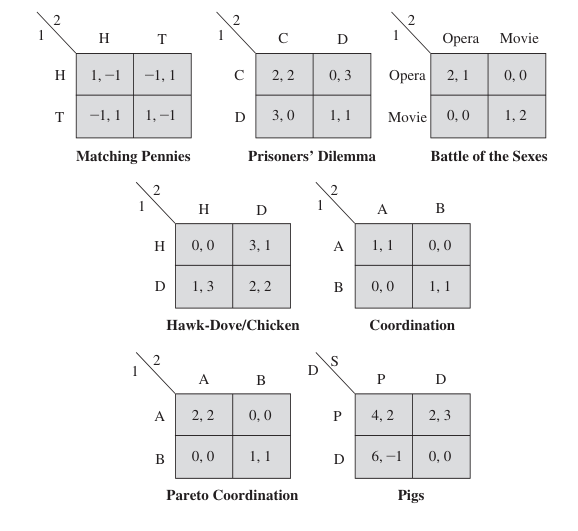
\includegraphics[scale=0.7]{images/2023-10-10-game_theory_04a.png}
\end{figure}

Note: Going from extensive-form to normal-form is always possible (just follow all paths and write down the payoff vector). Going from a normal-form to extensive form is more difficult as the relation is not 1:1; ie. more than one extensive-form representation has the same normal-form representation.


%%% Local Variables:
%%% mode: latex
%%% TeX-master: "journal"
%%% End:
